\documentclass[11pt]{article}

\usepackage[margin=1in]{geometry}
\usepackage{amsmath, amssymb}
\usepackage{booktabs}
\usepackage{graphicx}
\usepackage{hyperref}
\usepackage{siunitx}
\usepackage{enumitem}

\graphicspath{{report_figures/}}
\setlength{\emergencystretch}{2em}

\title{Identifying Neural Fingerprints from Visual-Evoked EEG: A Time-Frequency BCI Biometrics Study}
\author{
Dennis Sun, Evelyn Zhang, Qirui Zheng, and Yixuan Xin\\
\small Department of Cognitive Science, University of California San Diego
}
\date{April 27, 2026}

\begin{document}
\maketitle

\begin{abstract}
This project investigates whether subject identity can be decoded from visual-evoked electroencephalography (EEG) responses and, more specifically, which component of the signal carries the biometric ``neural fingerprint.'' The dataset comes from a rapid visual image presentation paradigm, in which subjects viewed different image categories while EEG was recorded over posterior visual electrodes. The initial hypothesis was category-based: if different image classes evoke distinct responses, then subject identity might be mediated by semantic or visual-category processing. However, representational and classification analyses did not support this explanation. Instead, downstream wavelet and machine-learning experiments showed that identity is primarily encoded in subject-specific local time-frequency structure within visual-evoked responses, including stable ERP morphology and Alpha/Beta-range oscillatory features. Discrete wavelet transform (DWT) features improved classification over power spectral density (PSD) baselines, and a final fragmented-signal SVM experiment showed that even short random EEG windows retained strong subject-identifying information. These results suggest that EEG biometrics in this setting rely less on stimulus category and more on stable, individual-specific temporal microstructure in posterior visual responses.
\end{abstract}

\section{Introduction}

Brain-computer interface (BCI) biometrics asks whether neural recordings can serve as reliable identity signals. Unlike conventional biometrics such as face or fingerprint recognition, EEG-based identity markers are internal, dynamic, and affected by both neural processing and measurement noise. The central question in this project is therefore not only whether subjects can be classified from EEG, but also what part of the EEG signal makes such classification possible.

The source experiment used rapid visual image presentation. Because subjects viewed different visual categories, the first working hypothesis was that image category responses might explain the observed subject differences. In other words, the project initially asked whether a subject's neural fingerprint was mediated by differential responses to semantic visual content. Analyses based on spectrograms and representational similarity matrices did not provide strong support for this category hypothesis. Later analyses shifted the focus from image semantics to signal structure. The final evidence indicates that the relevant biometric information is better described as stable, subject-specific structure in visual-evoked EEG: information that is not explained by the image category itself, but remains highly discriminative across people.

\section{Data and Preprocessing}

The project pipeline converted raw EEG recordings into standardized preprocessed epoch tensors,
\begin{equation}
    X \in \mathbb{R}^{N \times C \times T},
\end{equation}
where $N$ is the number of trials, $C$ is the number of selected visual electrodes, and $T$ is the number of time samples per epoch. The main analyses used posterior visual channels such as O1, Oz, O2, POz, PO7, and PO8, consistent with the visual-evoked nature of the task.

The preprocessing pipeline segmented EEG around visual stimulus events, retained visual-cortex channels, and produced balanced subject-level tensors. The final full DWT feature dataset contained 20,000 samples from 10 subjects, with 2,000 samples per subject and 240 wavelet-derived features per trial.

\begin{figure}[htbp]
\centering
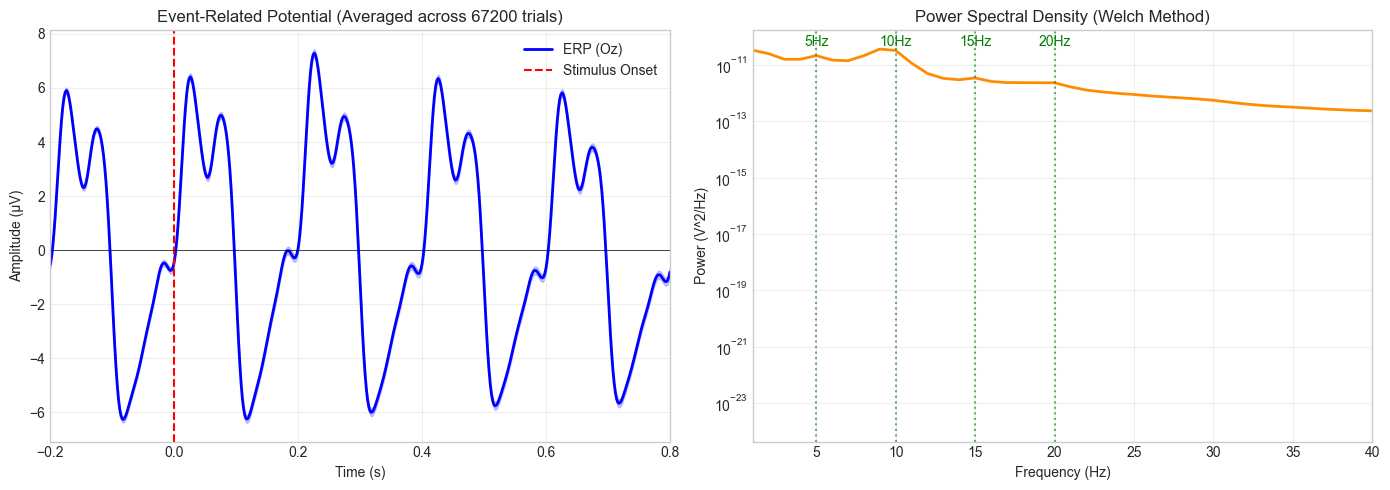
\includegraphics[width=0.92\linewidth]{fig01_signal_quality.png}
\caption{Signal-quality inspection from the preprocessing pipeline. This diagnostic visualization verifies that the extracted visual-evoked EEG epochs contain structured ERP and spectral content before downstream feature extraction.}
\label{fig:signal-quality}
\end{figure}

\begin{figure}[htbp]
\centering
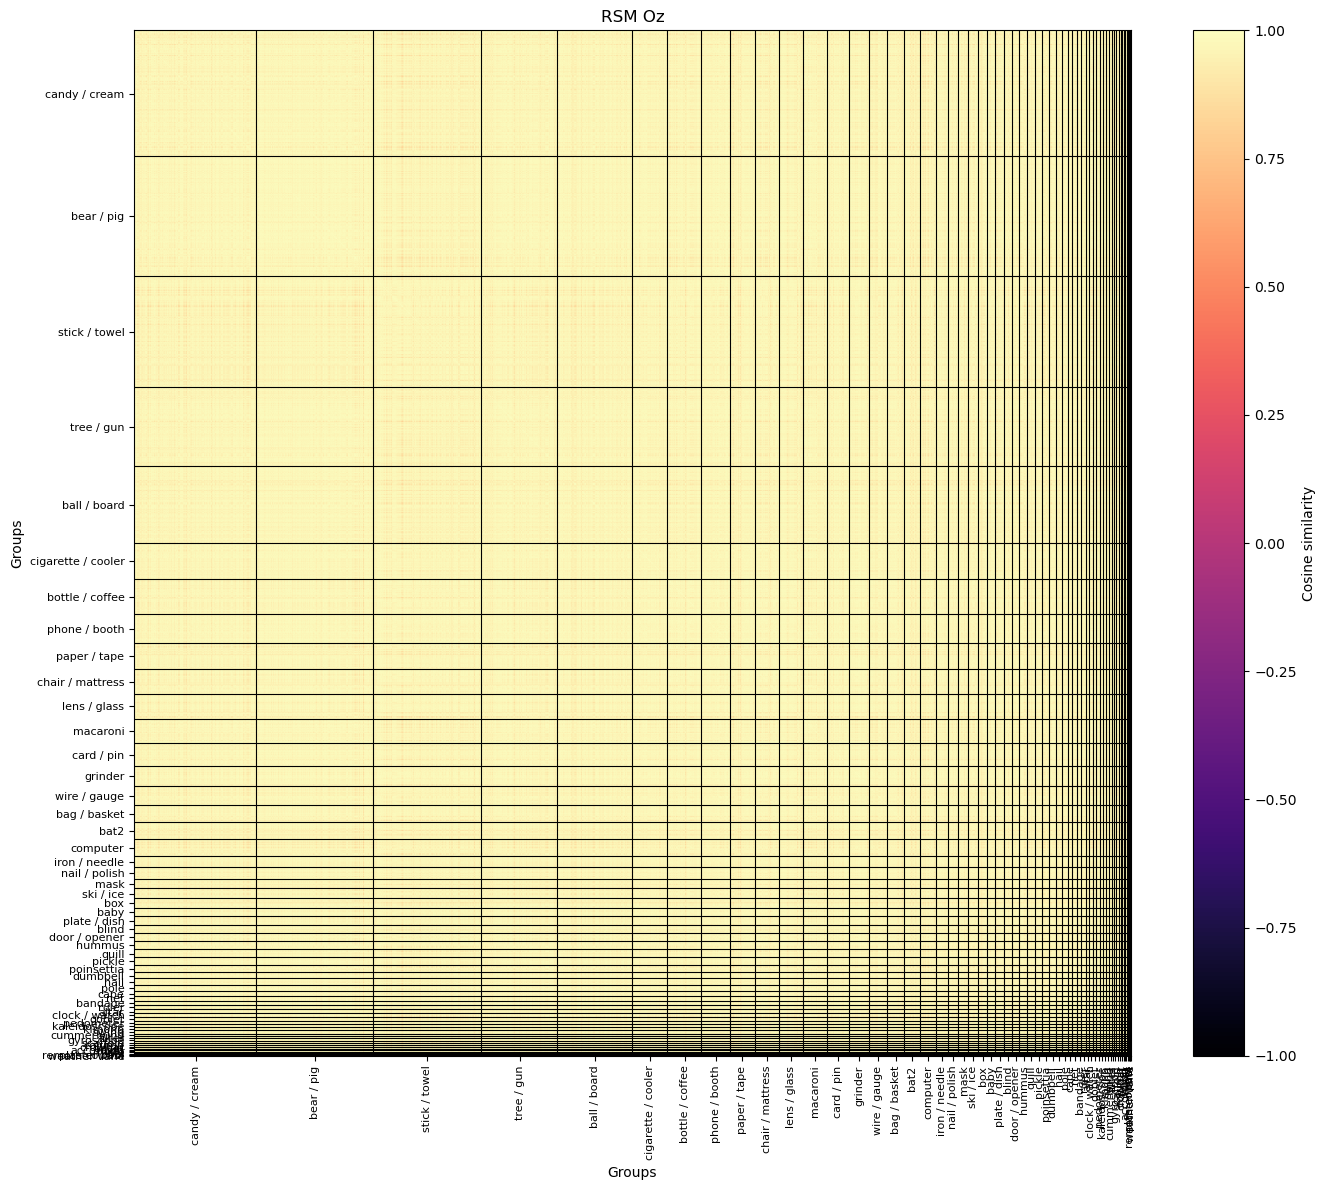
\includegraphics[width=0.78\linewidth]{fig03_oz_rsm.png}
\caption{Representative representational similarity matrix from the spectrogram/category analysis at channel Oz. The category-level analysis motivated the original image-category hypothesis, but later classification and ablation experiments showed that semantic category was not the primary driver of biometric separability.}
\label{fig:oz-rsm}
\end{figure}

\section{Feature Extraction}

\subsection{PSD Baseline}

The initial baseline used power spectral density (PSD) features. PSD measures static frequency-domain energy and is useful as a simple BCI baseline, but it collapses temporal dynamics within the epoch. Logistic Regression on PSD features reached approximately $80.83\%$ accuracy, confirming that frequency power carries identity information but leaving substantial room for improvement.

\subsection{Discrete Wavelet Transform Features}

To preserve local temporal structure, the project used the discrete wavelet transform (DWT). For each trial, channel, and wavelet band, five statistics were computed:
\begin{equation}
    \phi(x)=\{\mathrm{energy}, \log(\mathrm{energy}), \mu, \sigma, H\}_{\mathrm{channel}\times\mathrm{band}},
\end{equation}
where $\mu$ is the coefficient mean, $\sigma$ is the coefficient standard deviation, and $H$ is Shannon entropy over normalized wavelet-coefficient energy. This representation preserves spatial, spectral, and local temporal information.

\begin{figure}[htbp]
\centering
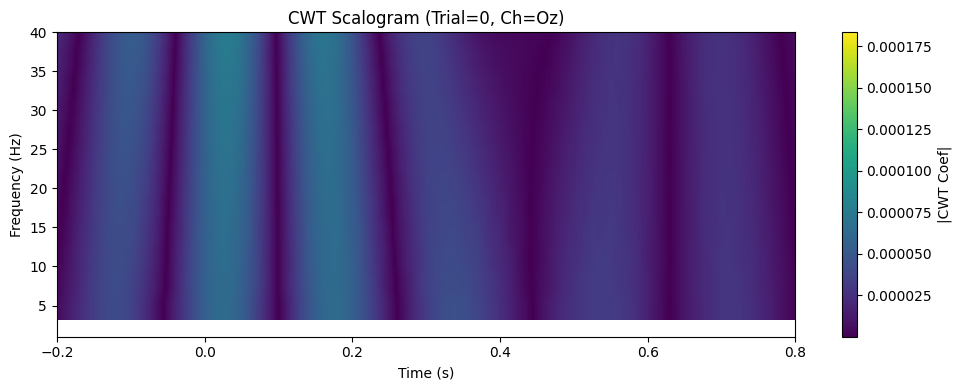
\includegraphics[width=0.86\linewidth]{fig04_cwt_scalogram.png}
\caption{Example time-frequency representation from the wavelet analysis. The scalogram illustrates why wavelet features are appropriate for this task: they retain transient local structure that PSD features discard.}
\label{fig:cwt}
\end{figure}

\section{Classification Experiments}

\subsection{Full-Epoch Subject Identification}

The main DWT classification experiment used an 80/20 stratified train-test split across 10 subjects. The results are summarized in Table~\ref{tab:model-comparison}.

\begin{table}[h]
\centering
\caption{Full-epoch subject identification using DWT features.}
\label{tab:model-comparison}
\begin{tabular}{lc}
\toprule
Model & Accuracy \\
\midrule
Logistic Regression & $89.12\%$ \\
RBF-SVM & $82.05\%$ \\
Random Forest & $72.02\%$ \\
\bottomrule
\end{tabular}
\end{table}

The strongest model was Logistic Regression, which is notable because it is a linear classifier. This suggests that DWT features unfold the EEG identity information into a space where subject classes are largely linearly separable. The result also indicates that highly nonlinear models were not necessary once the appropriate time-frequency representation was used.

\begin{figure}[htbp]
\centering
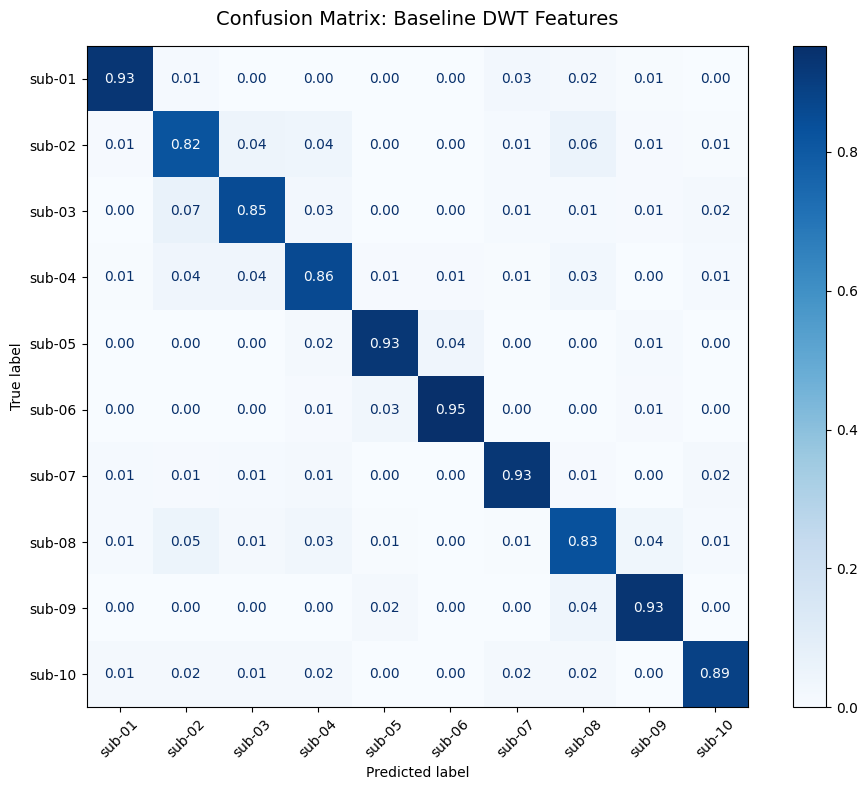
\includegraphics[width=0.72\linewidth]{fig05_dwt_confusion.png}
\caption{Baseline DWT Logistic Regression confusion matrix from the main machine-learning notebook. Most mass lies on the diagonal, supporting robust subject-level separability across all 10 participants.}
\label{fig:dwt-confusion}
\end{figure}

\subsection{Ablation Experiments}

Several ablation experiments tested whether the classifier relied on semantic category, phase-locked visual responses, or stable subject-specific structure. The main results are shown in Table~\ref{tab:ablation}.

\begin{table}[h]
\centering
\caption{Ablation results using Logistic Regression unless otherwise noted.}
\label{tab:ablation}
\begin{tabular}{lc}
\toprule
Condition & Accuracy \\
\midrule
Single-trial DWT baseline & $89.12\%$ \\
Trial-averaged ERP-enhanced condition & $94.97\%$ \\
Animals subset & $89.20\%$ \\
Objects subset & $88.92\%$ \\
Random pooled condition & $98.70\%$ \\
Chronological pooled split & $96.03\%$ \\
\bottomrule
\end{tabular}
\end{table}

The animals and objects subsets remained close to the full baseline, weakening the original image-category hypothesis. If semantic image class were the main driver, classification should have changed more strongly across category-specific subsets. Instead, identity remained recoverable regardless of category.

The trial-averaged and pooled conditions increased accuracy. This should not be interpreted as averaging suppressing the task-evoked ERP. In standard EEG analysis, time-domain averaging enhances phase-locked visual responses, including components such as P100 and N200, and attenuates non-phase-locked background activity. Therefore, the improvement after averaging suggests that the biometric signal is embedded in the stable, individual-specific shape of the visual ERP and in consistent oscillatory structure, rather than in arbitrary background noise.

\begin{figure}[htbp]
\centering
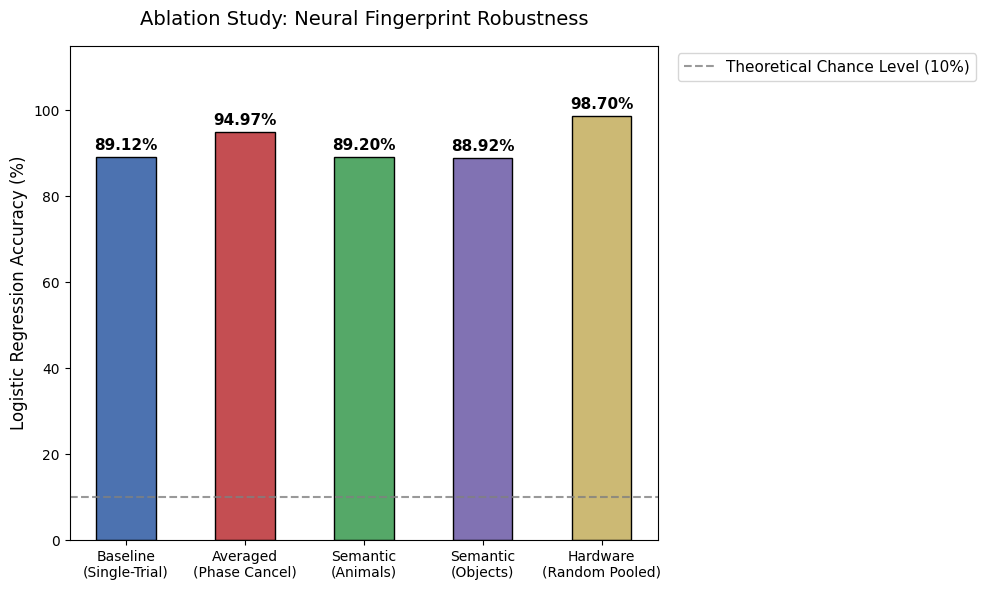
\includegraphics[width=0.86\linewidth]{fig05_ablation.png}
\caption{Ablation comparison across baseline, ERP-enhanced averaging, semantic subsets, and pooled conditions. The animals and objects subsets remain close to baseline, while averaging and pooling improve performance, shifting the interpretation away from image semantics and toward stable subject-specific visual-evoked signal structure.}
\label{fig:ablation}
\end{figure}

\section{Model Interpretation}

Logistic Regression coefficient analysis localized the strongest identity information to posterior visual electrodes, particularly O1, Oz, O2, PO7, and PO8. The most important wavelet bands were mid-scale bands such as D5, D4, and D3. Given the sampling rate and preprocessing band, these bands overlap strongly with canonical Alpha and Beta activity. This is physiologically plausible: individual differences in Alpha peak frequency, Alpha amplitude, and Alpha/Beta dynamics are well documented in EEG and are often stable across individuals. Across feature types, $\log(\mathrm{energy})$, mean, and standard deviation were more informative than entropy.

This pattern supports a physiological interpretation: the neural fingerprint is not a high-level semantic response to image content, but a stable subject-specific pattern in visual-evoked ERP morphology and Alpha/Beta-range oscillatory microstructure. It is spatially concentrated in visual cortex channels and temporally expressed through local wavelet-scale variation.

\begin{figure}[htbp]
\centering
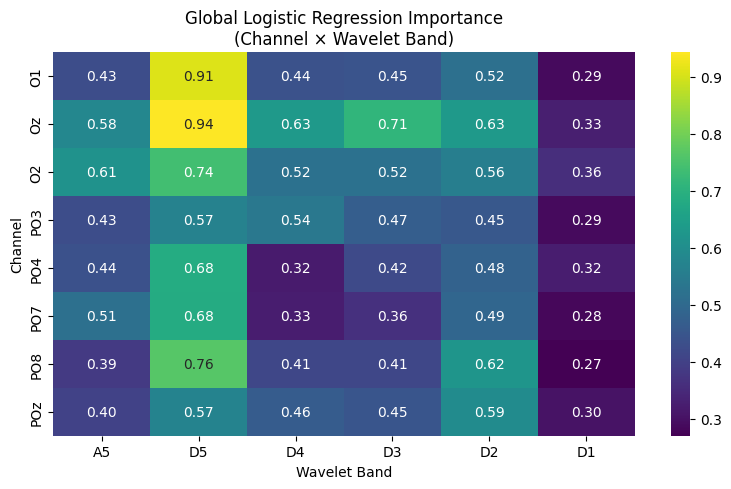
\includegraphics[width=0.78\linewidth]{fig05_feature_heatmap.png}
\caption{Global Logistic Regression coefficient importance aggregated by channel and wavelet band. The strongest weights concentrate in posterior visual electrodes and mid-scale Alpha/Beta-related wavelet bands, consistent with a visual-cortex time-frequency fingerprint.}
\label{fig:feature-heatmap}
\end{figure}

\section{Final Fragmented-Signal SVM Analysis}

The final experiment directly tested whether identity could be recovered from randomly fragmented EEG signals. Each subject's preprocessed EEG epochs were randomly cropped into short windows:
\begin{equation}
    x_i(t) \rightarrow x_i(t_s:t_s+L), \quad t_s \sim \mathrm{Uniform}(0,T-L).
\end{equation}
DWT features were extracted from each fragment, and SVM classifiers were trained to predict subject identity.

\begin{table}[h]
\centering
\caption{Reverse subject identification from random EEG fragments. Chance level is $10\%$.}
\label{tab:fragment}
\begin{tabular}{lcc}
\toprule
Fragment Length & RBF-SVM Accuracy & Linear-SVM Accuracy \\
\midrule
\SI{0.25}{s} & $55.90\%$ & $57.00\%$ \\
\SI{0.50}{s} & $67.57\%$ & $71.27\%$ \\
\SI{1.00}{s} & $81.53\%$ & $85.77\%$ \\
\bottomrule
\end{tabular}
\end{table}

The fragment experiment is the strongest evidence for distributed biometric structure. Even a \SI{0.25}{s} fragment classified subjects far above the $10\%$ chance level, and the best \SI{1.00}{s} Linear-SVM reached $85.77\%$. A permutation control with 20 shuffled-label repetitions returned to chance, with mean accuracy $10.12\%$ and standard deviation $0.37\%$. Thus, the fragment performance cannot be explained by class imbalance or an accidental split artifact.

\begin{figure}[htbp]
\centering
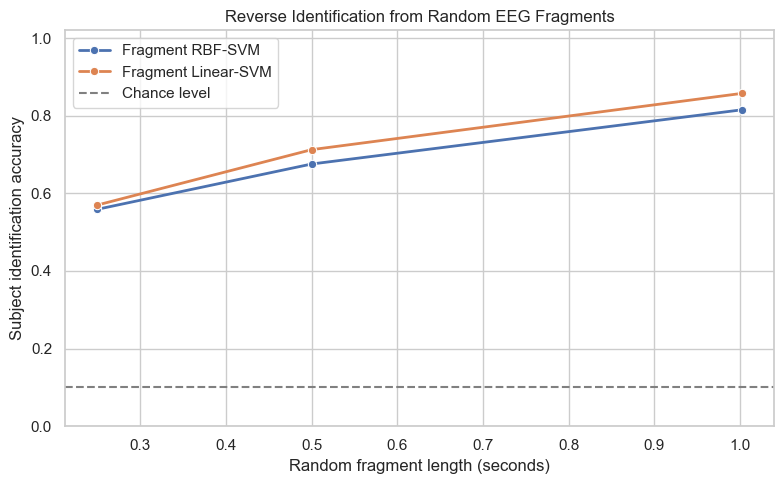
\includegraphics[width=0.78\linewidth]{fig06_fragment_curve.png}
\caption{Reverse identification accuracy from randomly cropped EEG fragments. Accuracy increases with fragment duration and remains far above the $10\%$ chance level even at \SI{0.25}{s}.}
\label{fig:fragment-curve}
\end{figure}

\begin{figure}[htbp]
\centering
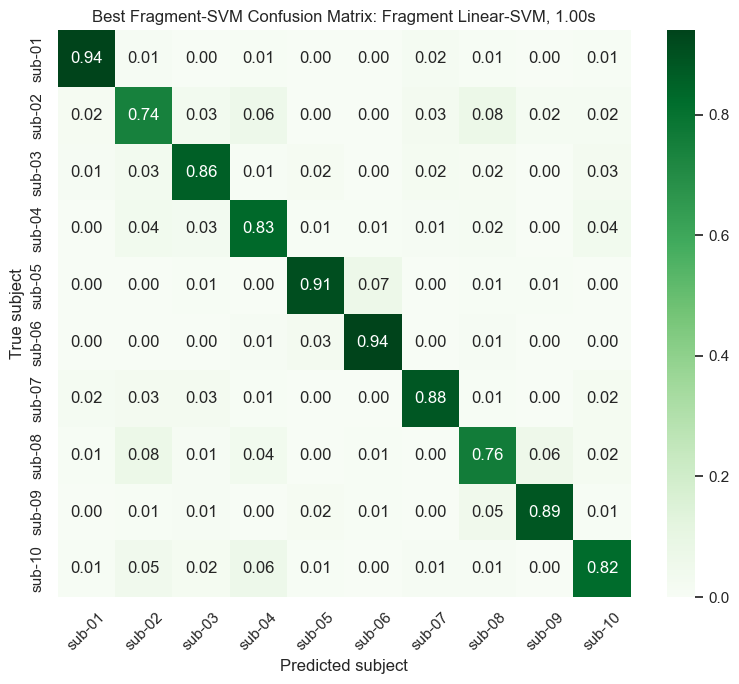
\includegraphics[width=0.72\linewidth]{fig06_fragment_confusion.png}
\caption{Best fragmented-signal SVM confusion matrix. The fragment-level classifier retains a diagonal-dominant structure, showing that identity information is distributed across local windows rather than only present in full epochs.}
\label{fig:fragment-confusion}
\end{figure}

\begin{table}[htbp]
\centering
\caption{Permutation control for the best fragmented-signal setting.}
\label{tab:permutation}
\begin{tabular}{lc}
\toprule
Condition & Accuracy \\
\midrule
Best true-label fragment model & $85.77\%$ \\
Permutation mean, 20 repetitions & $10.12\%$ \\
Permutation standard deviation & $0.37\%$ \\
Theoretical chance level & $10.00\%$ \\
\bottomrule
\end{tabular}
\end{table}

\section{Confusion-Matrix and Signal-Level Analysis}

The full-epoch DWT Logistic Regression model achieved $89.12\%$ accuracy. Per-subject recall ranged from $82.00\%$ for sub-02 to $95.25\%$ for sub-06. Errors were not uniformly distributed. The strongest mutual confusion occurred between sub-02 and sub-03, with 44 total cross-errors. Other notable confusions included sub-02 versus sub-08 and sub-02 versus sub-04.

\begin{figure}[htbp]
\centering
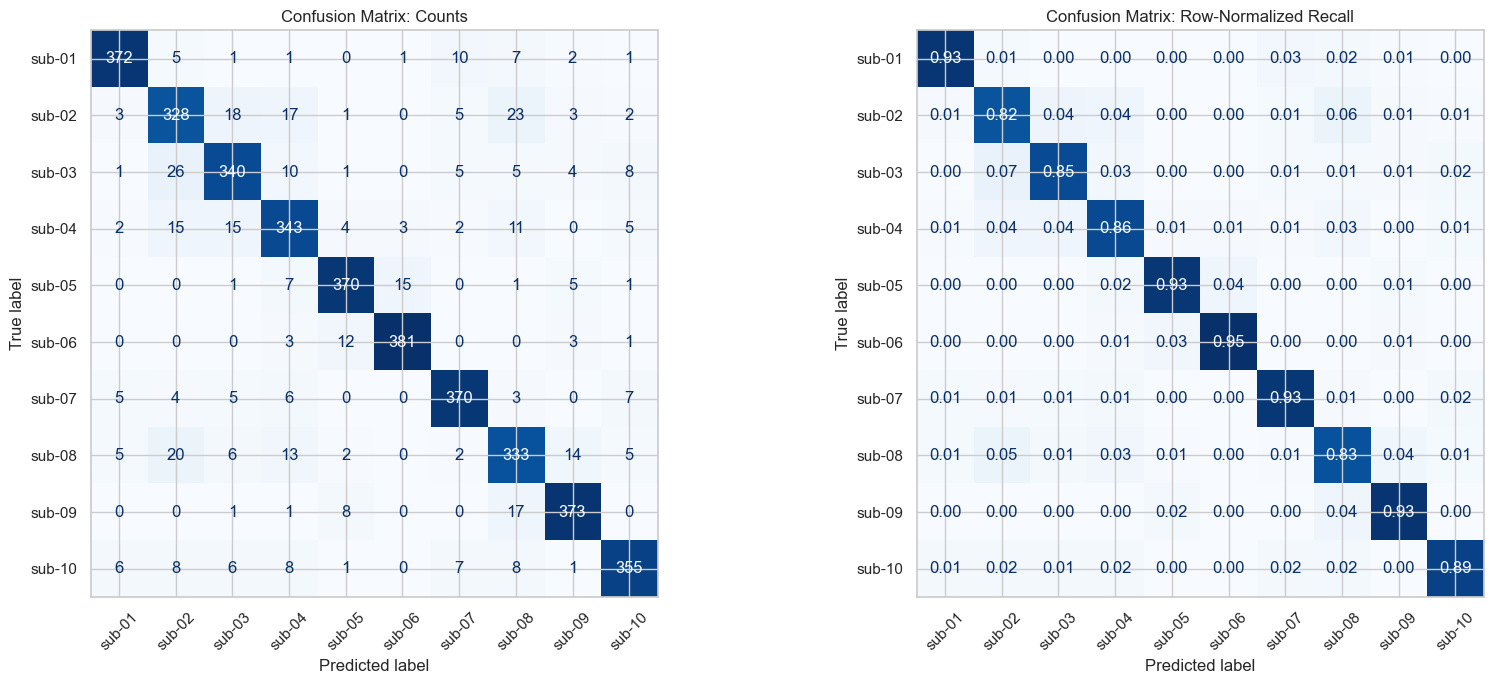
\includegraphics[width=0.92\linewidth]{fig06_confusion_detail.png}
\caption{Detailed count and row-normalized confusion matrices from the final analysis notebook. The error structure is concentrated in a small number of subject pairs rather than evenly spread across all classes.}
\label{fig:confusion-detail}
\end{figure}

\begin{table}[htbp]
\centering
\caption{Most important pairwise confusion outcomes from the final diagnostic analysis.}
\label{tab:confusion-summary}
\begin{tabular}{lcc}
\toprule
Diagnostic & Subject(s) & Value \\
\midrule
Easiest subject by recall & sub-06 & $95.25\%$ \\
Hardest subject by recall & sub-02 & $82.00\%$ \\
Strongest mutual confusion & sub-02 vs. sub-03 & 44 cross-errors \\
Second strongest mutual confusion & sub-02 vs. sub-08 & 43 cross-errors \\
\bottomrule
\end{tabular}
\end{table}

ERP comparison provided an additional signal-level view. The most confused pair, sub-02 and sub-03, had an ERP RMS distance of approximately $4.196\times 10^{-6}$ and flattened waveform correlation of $-0.2181$. Although the correlation value does not alone explain the classifier behavior, the pair-level analysis shows that misclassifications are structured and subject-pair specific rather than evenly random across all identities.

\begin{figure}[htbp]
\centering
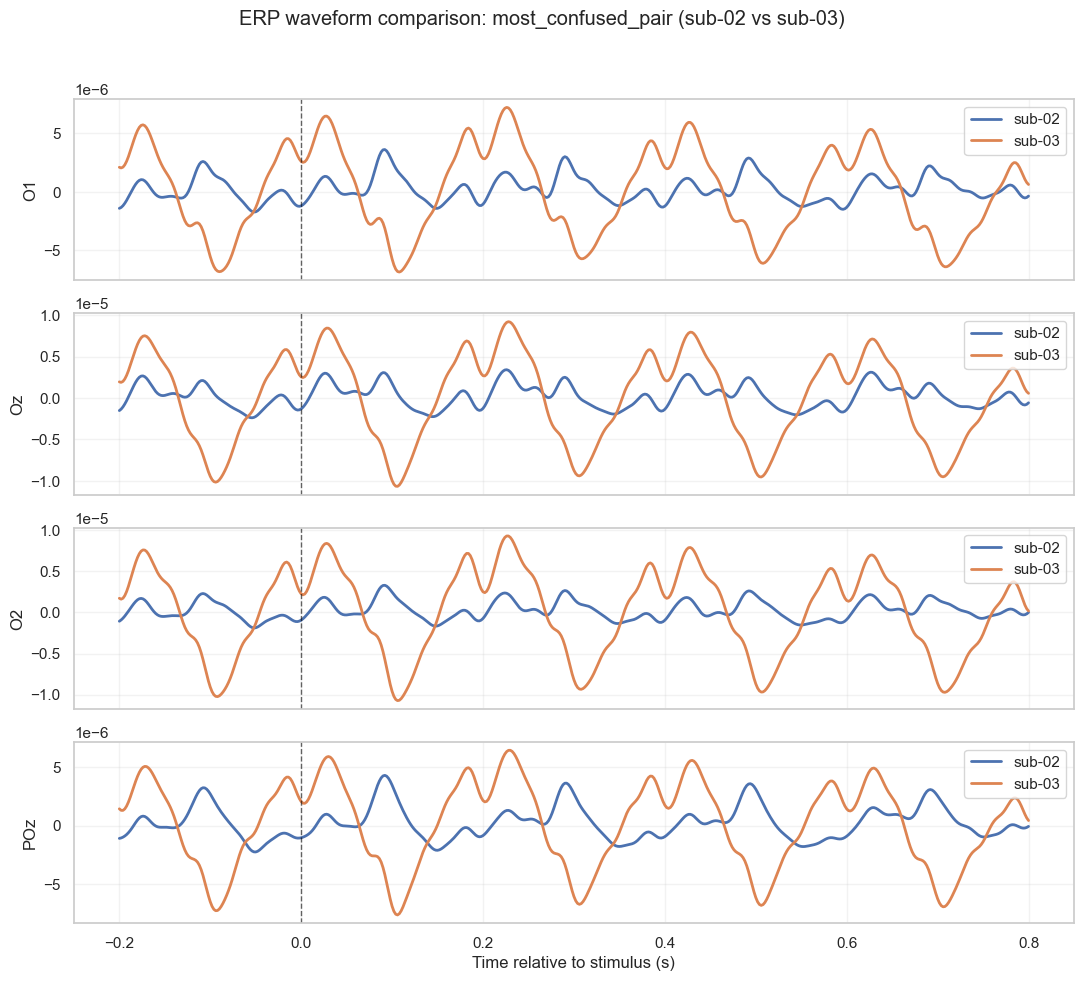
\includegraphics[width=0.88\linewidth]{fig06_erp_confused_pair.png}
\caption{ERP waveform comparison for the most confused subject pair, sub-02 and sub-03, across posterior visual channels. This signal-level view complements the confusion-matrix diagnosis by connecting classification errors to subject-pair waveform structure.}
\label{fig:erp-confused}
\end{figure}

\section{Discussion}

The main conceptual shift in this project is from a semantic-image hypothesis to a signal-microstructure hypothesis. The dataset's visual paradigm initially suggested that category-level visual processing might determine the biometric fingerprint. However, category-specific analyses showed that animals and objects produced nearly identical subject-identification performance. Therefore, image content is unlikely to be the decisive factor.

The stronger explanation is that each subject contributes a stable, individual-specific pattern to the visual EEG response. This pattern is not random measurement noise; it is more plausibly a mixture of subject-specific ERP morphology and Alpha/Beta oscillatory dynamics. Figures~\ref{fig:ablation}, \ref{fig:feature-heatmap}, and \ref{fig:fragment-curve} summarize this shift: category-specific subsets do not eliminate identity decoding, posterior wavelet features carry the strongest weights, and short fragments remain classifiable far above chance. DWT features expose this structure because they preserve local time-frequency variation. The fragment-SVM results further show that identity evidence is distributed across short signal windows rather than being restricted to a single full-epoch ERP shape.

This finding is important for BCI biometrics. It suggests that identity decoding can succeed even without explicit task semantics and even from partial EEG segments. At the same time, it raises methodological caution: features that are irrelevant to image-category decoding can still contain strong subject-level physiological information. Future BCI systems should distinguish between task-relevant neural responses and subject-specific biometric signatures, especially when generalization across users is required.

\section{Limitations}

The current project used 10 subjects and focused on posterior visual electrodes. Larger subject pools are needed to test scalability. The fragment-SVM experiment used random fragments from the available preprocessed data, but future work should evaluate stricter session-to-session transfer and cross-day stability. This is especially important because the waveform mean, a mean-level/DC-offset-like feature, was one of the informative feature types. In EEG, mean-level shifts can partially reflect true slow physiological variation, but they can also be affected by electrode impedance, cap placement, skin properties, and same-day recording setup. Therefore, the present results show strong within-session biometric separability, but they do not yet prove that every discriminative component is purely neural or stable across days.

\section{Conclusion}

This project demonstrates that visual-evoked EEG contains a robust neural fingerprint for subject identification. The original image-category hypothesis was not supported: semantic stimulus class did not determine the identity signal. Instead, the decisive information lies in subject-specific local time-frequency structure, concentrated in posterior visual electrodes and exposed by DWT features. Full-epoch DWT classification reached $89.12\%$, pooled and averaged variants improved performance further, and fragmented-signal SVM decoding reached $85.77\%$ with \SI{1.00}{s} windows while permutation controls returned to chance. These findings support the conclusion that EEG biometric identity is carried by stable visual-evoked ERP and Alpha/Beta-range oscillatory microstructure, with an important caveat that cross-session validation is needed to separate purely neural identity markers from recording-setup effects.

\end{document}
